\documentclass[tikz,border=10pt]{standalone}
\usepackage{tikz}
\usepackage{verbatim}
\begin{document}


\tikzset{every picture/.style={line width=0.75pt}} %set default line width to 0.75pt

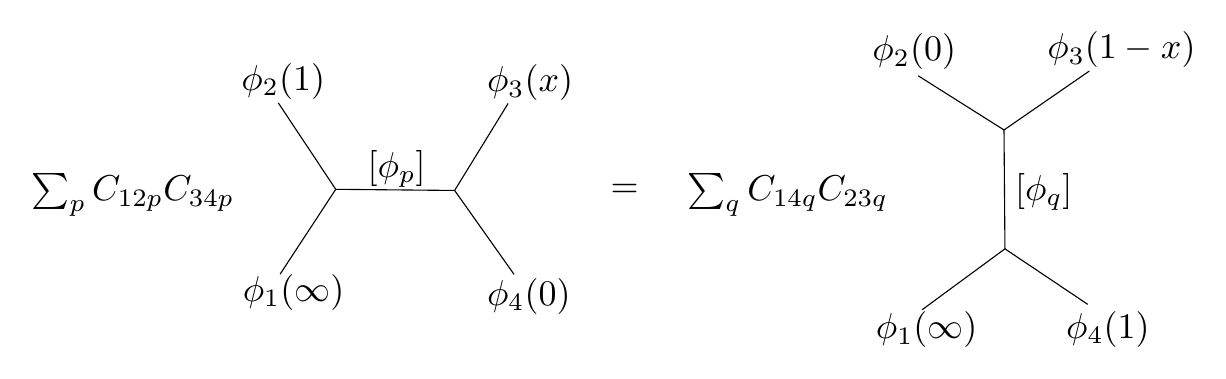
\begin{tikzpicture}[x=0.75pt,y=0.75pt,yscale=-1,xscale=1]
%uncomment if require: \path (0,300); %set diagram left start at 0, and has height of 300

%Straight Lines [id:da0115234795706054]
\draw    (146.51,87.96) -- (174.16,129.55) ;
%Straight Lines [id:da0884359191436006]
\draw    (174.16,129.55) -- (147.37,170.4) ;
%Straight Lines [id:da29958252277349096]
\draw    (174.16,129.55) -- (231.44,130.1) ;
%Straight Lines [id:da26570559949261296]
\draw    (260.09,170.55) -- (231.44,130.1) ;
%Straight Lines [id:da2509913784247453]
\draw    (231.44,130.1) -- (257.21,88.19) ;
%Straight Lines [id:da20046760050602686]
\draw    (537.22,72.58) -- (496.13,100.95) ;
%Straight Lines [id:da6638911580887084]
\draw    (496.13,100.95) -- (454.81,74.88) ;
%Straight Lines [id:da4526182308247384]
\draw    (496.13,100.95) -- (496.58,158.23) ;
%Straight Lines [id:da9348236571440502]
\draw    (456.65,187.59) -- (496.58,158.23) ;
%Straight Lines [id:da31525979015487127]
\draw    (496.58,158.23) -- (536.5,185) ;

% Text Node
\draw (127.73,168.98) node [anchor=north west][inner sep=0.75pt,scale=1.3]   {$\phi _{1}( \infty )$};
% Text Node
\draw (127.1,67.06) node [anchor=north west][inner sep=0.75pt,scale=1.3]   {$\phi _{2}( 1)$};
% Text Node
\draw (245.4,67.94) node [anchor=north west][inner sep=0.75pt,scale=1.3]   {$\phi _{3}( x)$};
% Text Node
\draw (245.4,170.74) node [anchor=north west][inner sep=0.75pt,scale=1.3]   {$\phi _{4}( 0)$};
% Text Node
\draw (187.85,109.24) node [anchor=north west][inner sep=0.75pt,scale=1.3]   {$[ \phi _{p}]$};
% Text Node
\draw (499.85,120.24) node [anchor=north west][inner sep=0.75pt,scale=1.3]   {$[ \phi _{q}]$};
% Text Node
\draw (432.73,186.98) node [anchor=north west][inner sep=0.75pt,scale=1.3]   {$\phi _{1}( \infty )$};
% Text Node
\draw (515.4,51.94) node [anchor=north west][inner sep=0.75pt,scale=1.3]   {$\phi _{3}( 1-x)$};
% Text Node
\draw (431.1,53.06) node [anchor=north west][inner sep=0.75pt,scale=1.3]   {$\phi _{2}( 0)$};
% Text Node
\draw (524.4,186.74) node [anchor=north west][inner sep=0.75pt,scale=1.3]   {$\phi _{4}( 1)$};
% Text Node
\draw (26,120.4) node [anchor=north west][inner sep=0.75pt,scale=1.3]   {$\sum _{p} C_{12p} C_{34p}$};
% Text Node
\draw (342,120.4) node [anchor=north west][inner sep=0.75pt,scale=1.3]   {$\sum _{q} C_{14q} C_{23q}$};
% Text Node
\draw (305,125.4) node [anchor=north west][inner sep=0.75pt,scale=1.3]   {$=$};


\end{tikzpicture}
\end{document}
